\mySection{5.8 Bayesian Estimation}
%-------------- start slide -------------------------------%{{{ 5.87
\begin{frame}
  % {\S\: 5.8 Bayesian Estimation}

{\bf Rationale:~} Let $W$ be an estimator dependent on a parameter $\theta$.
\begin{enumerate}
 \item Frequentists view $\theta$ as a parameter whose exact value is to be estimated.\\[1em]
 \item Bayesians view $\theta$ is the value of a random variable $\Theta$. \\[1em]
 \pause
 One can incorporate our knowledge on $\Theta$ --- the {\bf prior distribution} $p_\Theta(\theta)$ if $\Theta$ is discrete and $f_\Theta(\theta)$ if $\Theta$ is continuous --- and use Bayes' formula to update our knowledge on $\Theta$ upon new observation $W=w$:
%  \vfill
\begin{align*}
g_\Theta(\theta|W=w)=
\begin{cases}
 \displaystyle \frac{p_W(w|\Theta=\theta) p_\Theta(\theta)}{\PP(W=w)} & \text{if $W$ is discrete} \\[2em]
 \displaystyle \frac{f_W(w|\Theta=\theta) f_\Theta(\theta)}{f_W(w)}   & \text{if $W$ is continuous}
\end{cases}
 \end{align*}
 where $g_\Theta(\theta|W=w)$ is called {\bf posterior distribution} of $\Theta$.
\end{enumerate}
\end{frame}
%-------------- end slide -------------------------------%}}}
%-------------- start slide -------------------------------%{{{ 1
\begin{frame}[fragile]
\begin{center}
  \tikzset{every node/.append style={scale=0.9}}
  \tikzset{
      invisible/.style={opacity=0},
      visible on/.style={alt={#1{}{invisible} }},
      alt/.code args={<#1>#2#3}{%
        \alt<#1>{\pgfkeysalso{#2}}{\pgfkeysalso{#3}} % \pgfkeysalso doesn't change the path
      },
    }
  \tikzset{level 1 concept/.append style={font=\sf, sibling angle=90,level distance = 15em}}
  % \tikzset{level 2 concept/.append style={font=\sf, sibling angle=45,level distance = 15mm}}
  \begin{tikzpicture}[mindmap,concept color=black,text=black]

\def\colorTotal{red!80!black}
\def\colorPrior{green!80!black}
\def\colorL{yellow!80!black}
\def\colorPost{blue!80!black}
  \begin{scope}[concept color=red!30!black]
    \node[text width=14em,scale=1,text=white] (right) at (2.2,0) {$\Huge\displaystyle \textcolor{\colorPost}{P(\Theta|W)} = \frac{\textcolor{\colorL}{P(W\mid \Theta)}\textcolor{\colorPrior}{P(\Theta)}}{\textcolor{\colorTotal}{P(W)}}$}
    [counterclockwise from=45]
    child[concept color=\colorPrior] { node[concept] {Prior distribution of $\Theta$}}
    child[concept color=\colorL] { node[concept] {Likelihood of sample $W$} }
    child[concept color=\colorPost] { node[concept] {Posterior of $\Theta$} }
    child[concept color=\colorTotal] { node[concept] {Total Probability of sample $W$} }
  ;
  \end{scope}
  \end{tikzpicture}
\end{center}
\end{frame}
%-------------- end slide -------------------------------%}}}
%-------------- start slide -------------------------------%{{{ 5.88
 \begin{frame}{Four cases for computing posterior distribution}
 \begin{center}
 \def\arraystretch{4}
  \begin{tabular}{ l | c | c }
    \hline
  $g_\Theta(\theta|W=w)$ \cellcolor{gray!50!background} & $W$ discrete  \cellcolor{gray!50!background}                                                                             & $W$ continuous  \cellcolor{gray!50!background}                                                                          \\ \hline
  $\Theta$ discrete  \cellcolor{gray!50!background}     & $\displaystyle \frac{p_W(w|\Theta=\theta) p_\Theta(\theta)}{\sum_{i} p_W(w|\Theta=\theta_i) p_\Theta(\theta_i)}$         & $\displaystyle \frac{f_W(w|\Theta=\theta) p_\Theta(\theta)}{\sum_{i} f_W(w|\Theta=\theta_i) p_\Theta(\theta_i)}$        \\ \hline
  $\Theta$ continuous \cellcolor{gray!50!background}    & $\displaystyle \frac{p_W(w|\Theta=\theta) f_\Theta(\theta)}{\int_\R p_W(w|\Theta=\theta') f_\Theta(\theta')\ud \theta'}$ & $\displaystyle \frac{f_W(w|\Theta=\theta) f_\Theta(\theta)}{\int_\R f_W(w|\Theta=\theta') f_\Theta(\theta')\ud\theta'}$ \\ \hline
  \end{tabular}
\end{center}
\end{frame}
%-------------- end slide -------------------------------%}}}
%-------------- start slide -------------------------------%{{{ 5.89
\begin{frame}{Gamma distributions}
\[
\Gamma(r) := \int_0^\infty y^{r-1} e^{-y} \ud y,\quad r>0.
\] \pause
\vfill
Two parametrizations for {\bf Gamma distributions}:
\vfill
\begin{enumerate}
  \item With a \textcolor{magenta}{shape parameter} $r$ and a \textcolor{blue}{scale parameter} $\theta$:
 \[
 f_Y(y;r,\theta) =  \frac{y^{r-1} e^{-y/\theta}}{\theta^r \Gamma(r)},
 \qquad y>0, r,\theta>0.
 \]
 \vfill
 \item With a \textcolor{magenta}{shape parameter} $r$ and a \textcolor{yellow}{rate parameter} $\lambda=1/\theta$,
 \[
 f_Y(y;r,\lambda) = \frac{\lambda^r y^{r-1} e^{-\lambda y}}{\Gamma(r)},
 \qquad y>0, r,\lambda>0.
 \]
 \vfill
 \item[]
 \[
 \E[Y] =  \frac{r}{\lambda} = r\theta \quad \text{and}\quad
 \Var(Y) = \frac{r}{\lambda^2} = r\theta^2
 \]
\end{enumerate}

\end{frame}
%-------------- end slide -------------------------------%}}}
%-------------- start slide -------------------------------%{{{ 5.90
\begin{frame}[fragile]

 \begin{center}
  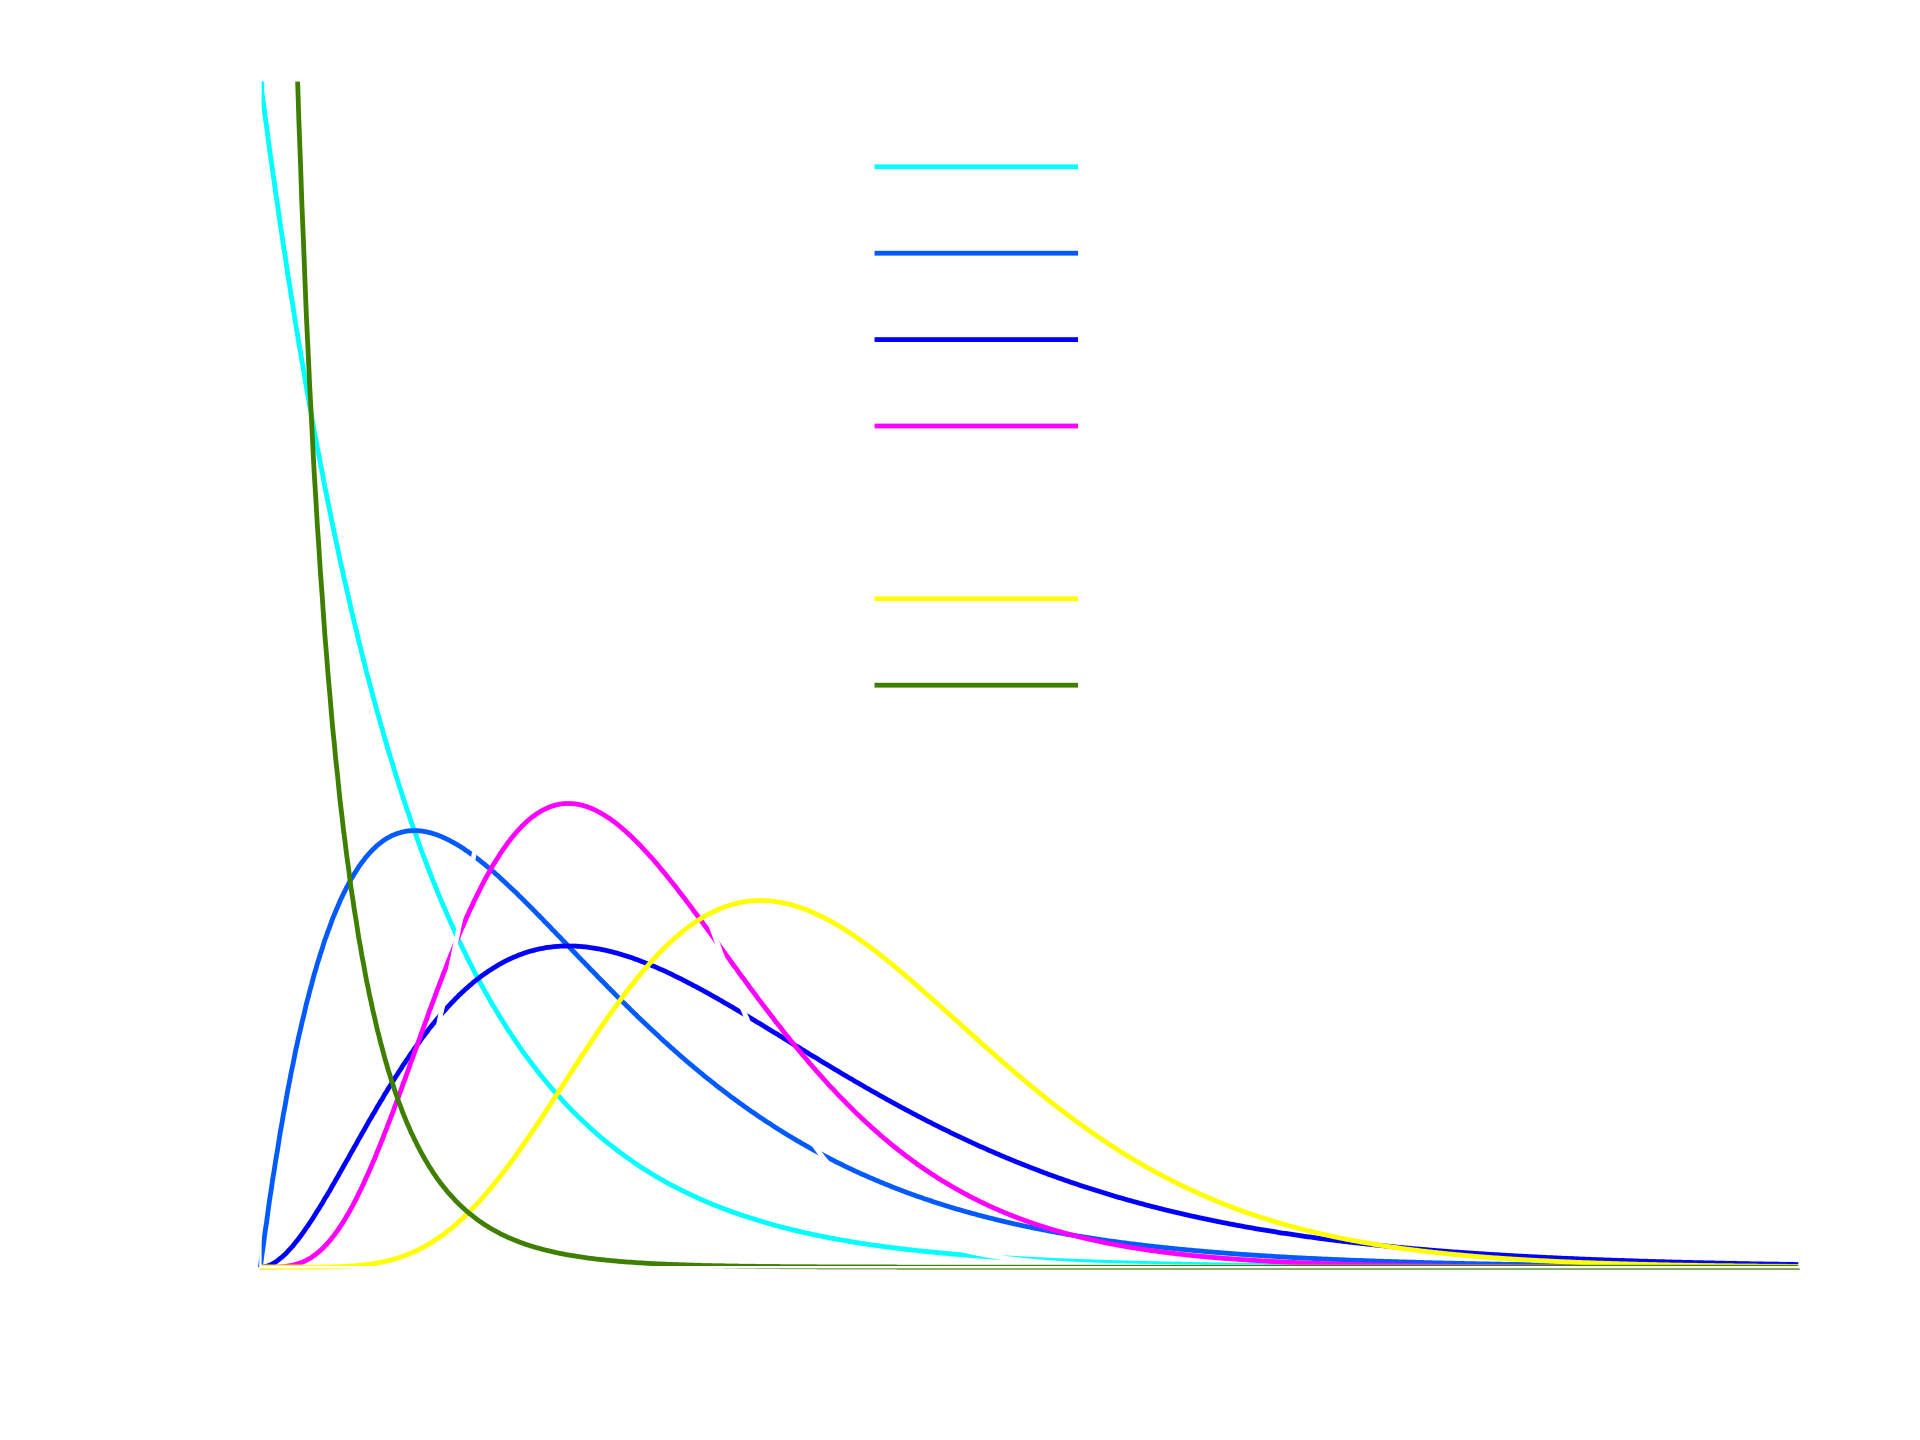
\includegraphics[scale=0.11]{1920px-Gamma_distribution_pdf.svg-neg.png}
  \begin{minipage}{0.4\textwidth}
  \begin{lstlisting}
# Plot gamma distributions
x = seq(0,20,0.01)
k= 3 # Shape parameter
theta = 0.5 # Scale parameter
plot(x,dgamma(x, k, scale = theta),
     type="l",
     col="red")
  \end{lstlisting}
  \end{minipage}
 \end{center}

\end{frame}
%-------------- end slide -------------------------------%}}}
%-------------- start slide -------------------------------%{{{ 5.91
\begin{frame}{Beta distributions}
 \begin{align*}
 B(\alpha,\beta) := & \int_0^1 y^{\alpha-1}(1-y)^{\beta-1}\ud y, \quad \alpha,\beta >0. \\ \pause
 \vdots& \qquad \vdots \\ \pause
 =& \frac{\Gamma(\alpha)\Gamma(\beta)}{\Gamma(\alpha+\beta)}. \qquad\qquad  \text{\textcolor{gray}{\small (see Appendix)}}
 \end{align*}
\vfill \pause
Beta distribution
\[
f_Y(y;\alpha,\beta) = \frac{y^{\alpha-1}(1-y)^{\beta-1}}{B(\alpha,\beta)}, \quad y\in[0,1], \alpha,\beta>0.
\]
\vfill \pause
\[
\E[Y] = \frac{\alpha}{\alpha+\beta}\quad\text{and}\quad
\Var(Y) = \frac{\alpha\beta}{(\alpha+\beta)^2(\alpha+\beta+1)}
\]
\end{frame}
%-------------- end slide -------------------------------%}}}
%-------------- start slide -------------------------------%{{{ 5.92
\begin{frame}[fragile]

\begin{center}
 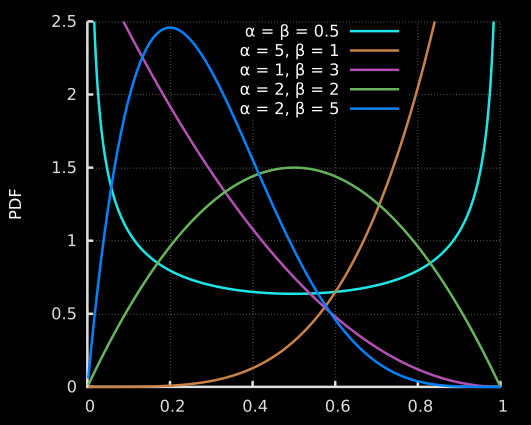
\includegraphics[scale=0.375]{Beta_distribution_pdf-neg.png}\\
 \vfill
 \begin{minipage}{0.4\textwidth}
  \begin{lstlisting}
   # Plot Beta distributions
x = seq(0,1,0.01)
a = 13
b = 2
plot(x,dbeta(x,a,b),
     type="l",
     col="red")
  \end{lstlisting}
 \end{minipage}
\end{center}

\end{frame}
%-------------- end slide -------------------------------%}}}
%-------------- start slide -------------------------------%{{{ 5.93
\begin{frame}
\begin{enumerate}
 \item[E.g. 1.]  Let $X_1,\cdots, X_n$ be a random sample from Bernoulli$(\theta)$: $p_{X_i}(k;\theta) = \theta^k(1-\theta)^{1-k}$ for $k=0,1$.\\[1em]  \pause
 Let $X=\sum_{i=1}^n X_i$. \pause
 Then $X$ follows binomial$(n, \theta)$. \\[1em] \pause
 Prior distribution: $\Theta\sim$beta$(r,s)$, i.e., $f_\Theta(\theta)=\frac{\Gamma(r+s)}{\Gamma(r)\Gamma(s)}\theta^{r-1}(1-\theta)^{s-1}$ for $\theta\in [0,1]$. \\ \pause
 \vfill
\begin{minipage}{0.45\textwidth}
\begin{eqnarray*}
 X_1,\cdots, X_n \:\big| \theta &\sim &\text{Bernoulli$(\theta)$}\\
 \Theta & \sim& \text{Beta$(r,s)$}\\
 && \text{$r$ \& $s$ are known}
\end{eqnarray*}
\end{minipage}
\hfill
\begin{minipage}{0.45\textwidth}
\begin{eqnarray*}
 X=\sum_{i=1}^nX_i \: \bigg| \theta&\sim& \text{Binomial$(n,\theta)$}\\
 \Theta & \sim& \text{Beta$(r,s)$}\\
 && \text{$r$ \& $s$ are known}
\end{eqnarray*}
\end{minipage}
\end{enumerate}
\end{frame}
%-------------- end slide -------------------------------%}}}
%-------------- start slide -------------------------------%{{{ 5.94
\begin{frame}
 \begin{center}
 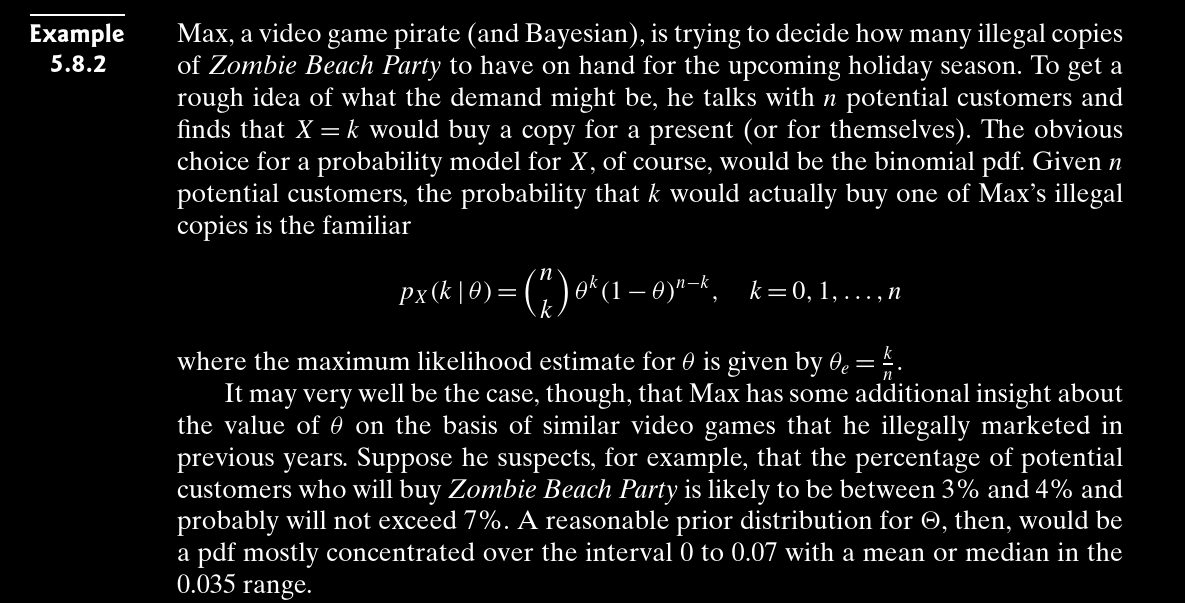
\includegraphics[scale=0.26]{Example-5-8-2-neg.png}
\end{center}
\end{frame}
%-------------- end slide -------------------------------%}}}
%-------------- start slide -------------------------------%{{{ 5.95
\begin{frame}
\begin{center}
 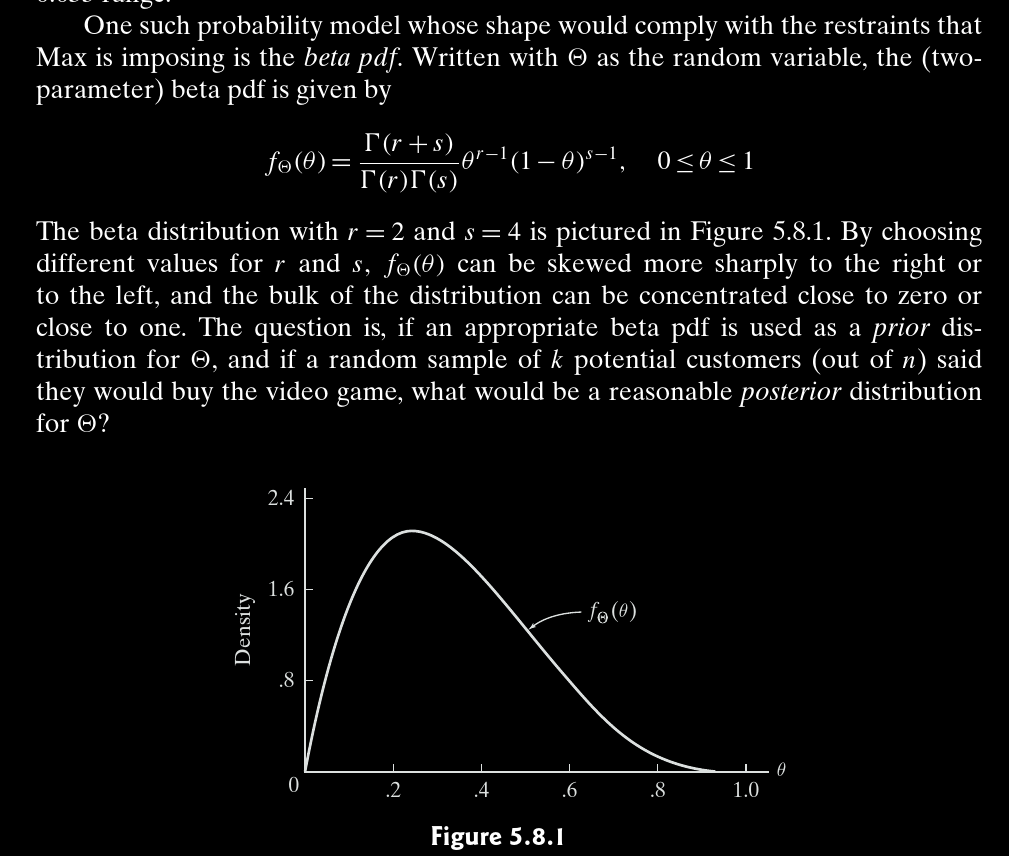
\includegraphics[scale=0.26]{Example-5-8-2-2-neg.png}
\end{center}

\end{frame}
%-------------- end slide -------------------------------%}}}
%-------------- start slide -------------------------------%{{{ 5.96
\begin{frame}
  $X$ is discrete and $\Theta$ is continuous.
  \[
 g_\Theta(\theta|X=k) = \frac{p_X(k|\Theta=\theta) f_\Theta(\theta)}{\int_\R p_X(k|\Theta=\theta') f_\Theta(\theta')\ud \theta'}
  \] \pause
  \begin{align*}
  p_X(k|\Theta=\theta) f_\Theta(\theta)
  &= {n\choose k} \theta^k (1-\theta)^{n-k} \times \frac{\Gamma(r+s)}{\Gamma(r)\Gamma(s)}\theta^{r-1}(1-\theta)^{s-1}\\ \pause
  &= {n\choose k} \frac{\Gamma(r+s)}{\Gamma(r)\Gamma(s)} \theta^{k+r-1} (1-\theta)^{n-k+s-1},\quad \theta\in[0,1].
  \end{align*}\pause
\begin{align*}
p_X(k) =& \int_\R p_X(k|\Theta=\theta') f_\Theta(\theta') \ud\theta'\\ \pause
=& {n\choose k} \frac{\Gamma(r+s)}{\Gamma(r)\Gamma(s)}  \int_0^1 \theta'^{k+r-1} (1-\theta')^{n-k+s-1}\ud \theta'\\ \pause
=& {n\choose k} \frac{\Gamma(r+s)}{\Gamma(r)\Gamma(s)}  \times \frac{\Gamma(k+r)\Gamma(n-k+s)}{\Gamma((k+r)+(n-k+s))}
\end{align*}
\end{frame}
%-------------- end slide -------------------------------%}}}
%-------------- start slide -------------------------------%{{{ 5.97
\begin{frame}
 \begin{align*}
  g_\Theta(\theta|X=k) =& \frac{\displaystyle {n\choose k} \frac{\Gamma(r+s)}{\Gamma(r)\Gamma(s)} \times \theta^{k+r-1} (1-\theta)^{n-k+s-1}}{\displaystyle {n\choose k} \frac{\Gamma(r+s)}{\Gamma(r)\Gamma(s)}  \times \frac{\Gamma(k+r)\Gamma(n-k+s)}{\Gamma((k+r)+(n-k+s))}} \\ \pause
  = & \frac{\Gamma(n+r+s)}{\Gamma(k+r)\Gamma(n-k+s)} \theta^{k+r-1} (1-\theta)^{n-k+s-1}, \qquad \theta\in[0,1]
 \end{align*} \pause
 \vfill
Conclusion: the posterior $\sim$ beta distribution$(k+r, n-k+s)$. \\[1em]
Recall that the prior $\sim$ beta distribution$(r, s)$.
\end{frame}
%-------------- end slide -------------------------------%}}}
%-------------- start slide -------------------------------%{{{ 5.98
\begin{frame}

It remains to determine the values of $r$ and $s$ to incorporate the prior knowledge: \\[1em]
\begin{enumerate}
 \item[PK 1.] Mean is about 0.035.
 \[
\E(\Theta) = 0.035 \quad\Longrightarrow\quad \frac{r}{r+s} = 0.035 \quad \Longleftrightarrow \quad \frac{r} {s}= \frac{7}{193}
\]
\vfill
\item[PK 2.] The pdf mostly concentrated over $[0,0.07]$. ... trial ...
\end{enumerate}
\end{frame}
%-------------- end slide -------------------------------%}}}
%-------------- start slide -------------------------------%{{{ 5.99
\begin{frame}[fragile]

\begin{minipage}{0.45\textwidth}
  \begin{lstlisting}
x <- seq(0, 1, length = 1025)
plot(x,dbeta(x,4,102),
     type="l")
plot(x,dbeta(x,7,193),
     type="l")
dev.off()

pdf=cbind(dbeta(x,4,102),dbeta(x,7,193))
matplot(x,pdf,
        type="l",
        lty = 1:2,
        xlab = "theta", ylab = "PDF",
        lwd = 2 # Line width
        )
legend(0.2, 25, # Position of legend
       c("Beta(4,102)", "Beta(7,193)"),
       col = 1:2, lty = 1:2,
       ncol = 1, # Number of columns
       cex = 1.5, # Fontsize
       lwd=2 # Line width
       )
abline(v=0.07, col="blue", lty=1,lwd=1.5)
text(0.07, -0.5, "0.07")
abline(v=0.035, col="gray60", lty=3,lwd=2)
text(0.035, 1, "0.035")
\end{lstlisting}
\end{minipage}
\begin{minipage}{0.5\textwidth}
  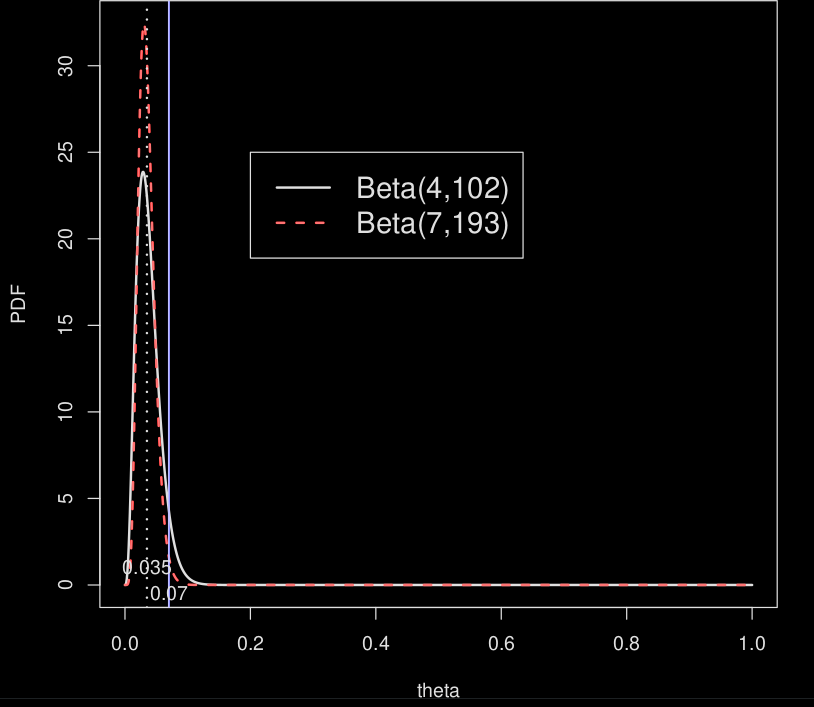
\includegraphics[scale=0.24]{BetaPrior_neg.png}
\end{minipage}
\end{frame}
%-------------- end slide -------------------------------%}}}
%-------------- start slide -------------------------------%{{{ 5.100
\begin{frame}
If we choose $r=7$ and $s=193$:
 \begin{align*}
  g_\Theta(\theta|X=k) = & \frac{\Gamma(n+200)}{\Gamma(k+7)\Gamma(n-k+193)} \theta^{k+6} (1-\theta)^{n-k+192}, \qquad \theta\in[0,1]
 \end{align*}
 \vfill
 Moreover, if $n=10$ and $k=2$,
  \begin{align*}
  g_\Theta(\theta|X=k) = & \frac{\Gamma(210)}{\Gamma(9)\Gamma(201)} \theta^{8} (1-\theta)^{200}, \qquad \theta\in[0,1]
 \end{align*}
\end{frame}
%-------------- end slide -------------------------------%}}}
%-------------- start slide -------------------------------%{{{ 5.101
\begin{frame}[fragile]

\begin{minipage}{0.45\textwidth}
 \begin{lstlisting}
x <- seq(0, 0.1, length = 1025)
pdf=cbind(dbeta(x,7,193),dbeta(x,9,201))
matplot(x,pdf,
        type="l",
        lty = 1:2,
        xlab = "theta", ylab = "PDF",
        lwd = 2 # Line width
)
legend(0.05, 25, # Position of legend
       c("Posterior Beta(9,201)", "Prior Beta(7,193)"),
       col = 1:2, lty = 1:2,
       ncol = 1, # Number of columns
       cex = 1.5, # Fontsize
       lwd=2 # Line width
)
abline(v=0.07,col="blue", lty=1,lwd=1.5)
text(0.07, -0.5, "0.07")
abline(v=0.035,col="black", lty=3,lwd=2)
text(0.035, 1, "0.035")
 \end{lstlisting}
\end{minipage}
\begin{minipage}{0.5\textwidth}
 \centering
 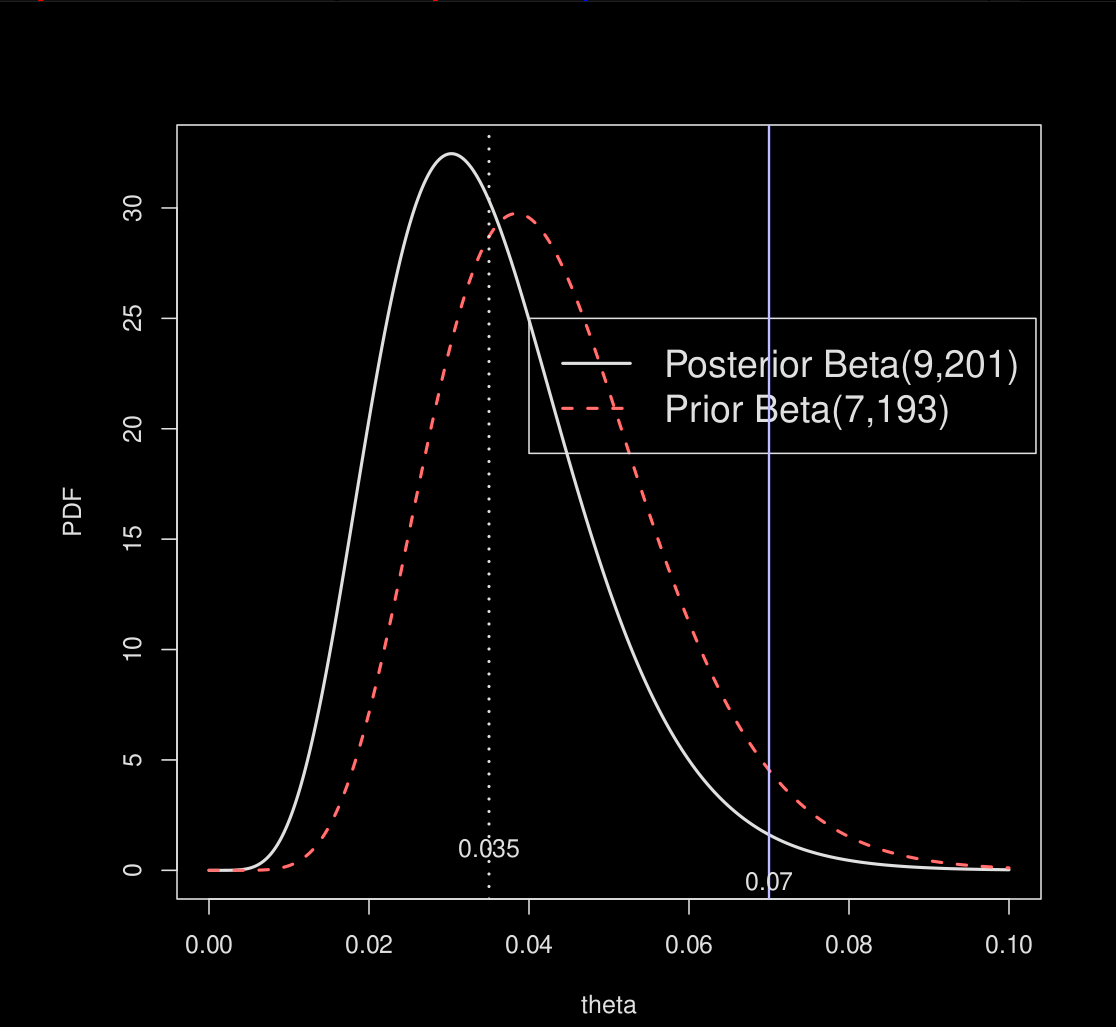
\includegraphics[scale=0.16]{BetaPriorPosterior_neg.png}
\end{minipage}
 \end{frame}

 \begin{frame}

 {\bf Definition.~} If the posterior distributions $p(\Theta| X)$ are in the same probability distribution family as the prior probability distribution $p(\Theta)$,
 the prior and posterior are then called \textcolor{magenta}{conjugate distributions}, and the prior is called a \textcolor{magenta}{conjugate prior} for the likelihood function.

 \vfill
 \begin{enumerate}
  \item Beta distributions are conjugate priors for Bernoulli, \underline{binomial}, nega. binomial, geometric  likelihood.
  \\[1em]
  \item Gamma distributions are conjugate priors for \underline{Poisson} and exponential likelihood.
 \end{enumerate}

\end{frame}
%-------------- end slide -------------------------------%}}}
%-------------- start slide -------------------------------%{{{ 5.102
\begin{frame}

\begin{enumerate}
 \item[E.g. 2.] Let $X_1,\cdots, X_n$ be a random sample from Poisson$(\theta)$: $p_X(k;\theta) = \frac{e^{-\theta}\theta^k}{k!}$ for $k=0,1,\cdots$.\\[1em]  \pause
 Let $W=\sum_{i=1}^n X_i$. \pause
 Then $W$ follows Poisson$(n\theta)$. \\[1em] \pause
 Prior distribution: $\Theta\sim$ Gamma$(s,\mu)$, i.e., $f_\Theta(\theta)=\frac{\mu^s}{\Gamma(s)}\theta^{s-1}e^{-\mu\theta}$ for $\theta>0$. \\[1em]\pause
%  Posterior Gamma$(w+s,\mu+n)$ upon observing $W=w$.
\end{enumerate}
\vfill
\begin{minipage}{0.45\textwidth}
\begin{eqnarray*}
 X_1,\cdots, X_n \:\big| \theta &\sim &\text{Poisson$(\theta)$}\\
 \Theta & \sim& \text{Gamma$(s,\mu)$}\\
 && \text{$s$ \& $\mu$ are known}
\end{eqnarray*}
\end{minipage}
\hfill
\begin{minipage}{0.45\textwidth}
\begin{eqnarray*}
 W=\sum_{i=1}^nX_i \: \bigg| \theta&\sim& \text{Poisson$(n\theta)$}\\
 \Theta & \sim& \text{Gamma$(s,\mu)$}\\
 && \text{$s$ \& $\mu$ are known}
\end{eqnarray*}
\end{minipage}
\end{frame}
%-------------- end slide -------------------------------%}}}
%-------------- start slide -------------------------------%{{{ 5.103
\begin{frame}
  \[
 g_\Theta(\theta|W=w) = \frac{p_W(w|\Theta=\theta) f_\Theta(\theta)}{\int_\R p_W(w|\Theta=\theta') f_\Theta(\theta')\ud \theta'}
  \]
  \vfill \pause
  \begin{align*}
  p_W(w|\Theta=\theta) f_\Theta(\theta)
  &= \frac{e^{-n\theta}(n\theta)^w}{w!}\times \frac{\mu^s}{\Gamma(s)}\theta^{s-1}e^{-\mu\theta}\\ \pause
  &= \frac{n^w}{w!} \frac{\mu^s}{\Gamma(s)}\times \theta^{w+s-1}e^{-(\mu+n)\theta}, \quad \theta>0.
  \end{align*}
\vfill \pause
  \begin{align*}
p_W(w) =& \int_\R p_W(w|\Theta=\theta') f_\Theta(\theta') \ud\theta'\\ \pause
=& \frac{n^w}{w!} \frac{\mu^s}{\Gamma(s)} \int_0^\infty \theta'^{w+s-1}e^{-(\mu+n)\theta'}\ud \theta'\\\pause
=& \frac{n^w}{w!} \frac{\mu^s}{\Gamma(s)} \times \frac{\Gamma(w+s)}{(\mu+n)^{w+s}}
\end{align*}
\end{frame}
%-------------- end slide -------------------------------%}}}
%-------------- start slide -------------------------------%{{{ 5.104
\begin{frame}
 \begin{align*}
  g_\Theta(\theta|X=k) =& \frac{\displaystyle \frac{n^w}{w!} \frac{\mu^s}{\Gamma(s)} \times \theta^{w+s-1}e^{-(\mu+n)\theta}}{\displaystyle  \frac{n^w}{w!} \frac{\mu^s}{\Gamma(s)} \times \frac{\Gamma(w+s)}{(\mu+n)^{w+s} }} \\
  = & \frac{(\mu+n)^{w+s}}{\Gamma(w+s)} \theta^{w+s-1}e^{-(\mu+n)\theta}, \qquad \theta>0.
 \end{align*}
 \vfill
Conclusion: the posterior of $\Theta$ $\sim$ gamma distribution$(w+s, n+\mu)$. \\[1em]
Recall that the prior of $\Theta$ $\sim$ gamma distribution$(s, \mu)$.
\end{frame}
%-------------- end slide -------------------------------%}}}
%-------------- start slide -------------------------------%{{{ 5.105
\begin{frame}[fragile]{Case Study 5.8.1}

 \begin{minipage}{0.45\textwidth}
 \begin{lstlisting}
x <- seq(0, 4, length = 1025)
pdf=cbind(dgamma(x, shape=88, rate=50),
          dgamma(x, shape=88+92, 100),
          dgamma(x, 88+92+72, 150))
matplot(x,pdf,
        type="l",
        lty = 1:3,
        xlab = "theta", ylab = "PDF",
        lwd = 2 # Line width
)
legend(2, 3.5, # Position of legend
       c("Prior Gamma(88,50)",
         "Posterior1 Beta(180,100)",
         "Posterior2 Beta(252,150)"),
       col = 1:3, lty = 1:3,
       ncol = 1, # Number of columns
       cex = 1.5, # Fontsize
       lwd=2 # Line width
)
 \end{lstlisting}
 \end{minipage}
\begin{minipage}{0.5\textwidth}
 \begin{center}
 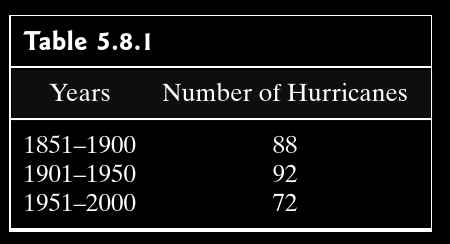
\includegraphics[scale=0.2]{Table-5-8-1-neg.png}
 \vspace{-2em}
 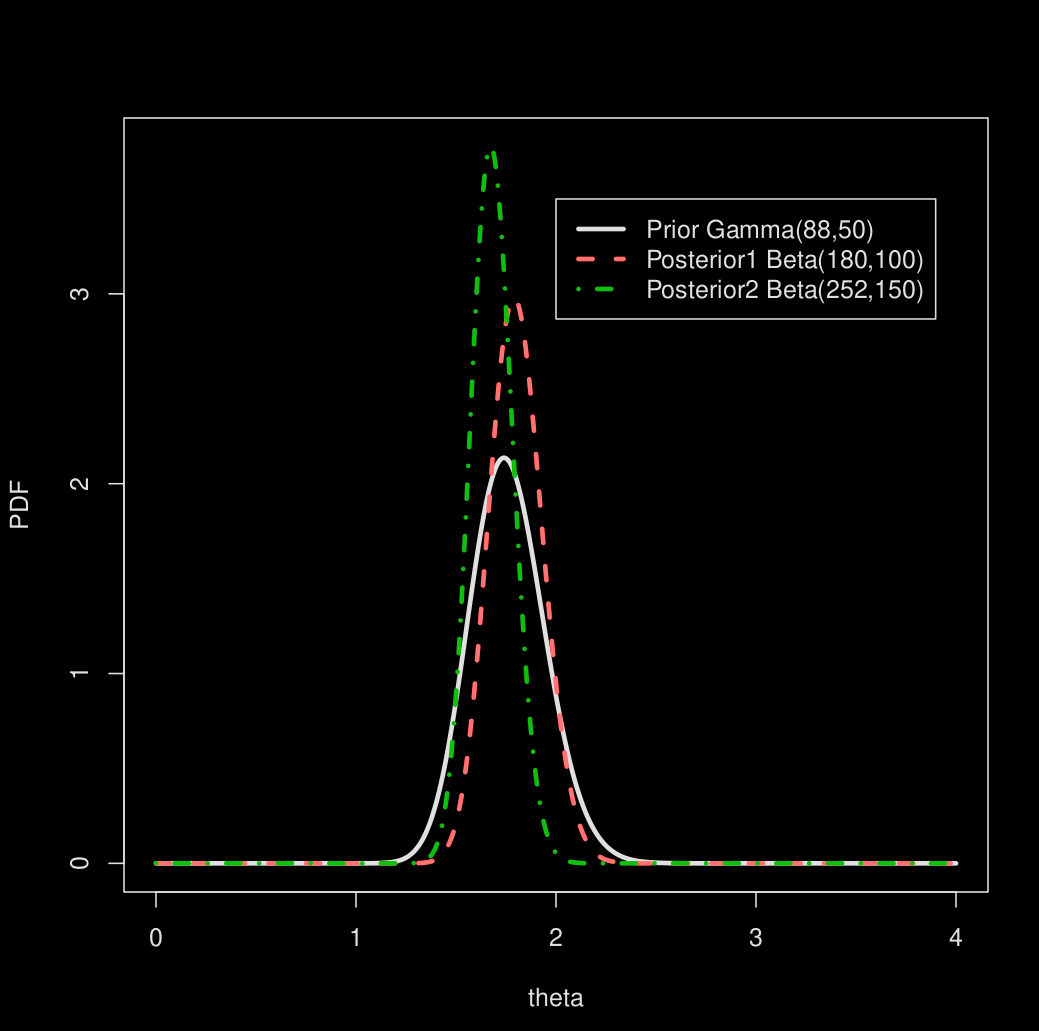
\includegraphics[scale=0.15]{GammaPriorPosterior_neg.png}
 \end{center}
\end{minipage}
\end{frame}
%-------------- end slide -------------------------------%}}}
%-------------- start slide -------------------------------%{{{ 5.106
\begin{frame}{Bayesian Point Estimation}

 {\bf Question.~} Can one calculate an appropriate {\em point estimate} $\theta_e$ given the posterior $g_\Theta(\theta|W=w)$?
 \vfill \pause
 {\bf Definitions.~}
Let $\theta_e$ be an estimate for $\theta$ based on a statistic $W$.
The \textcolor{magenta}{loss function} associated with $\theta_e$ is denoted $L(\theta_e,\theta)$, where $L(\theta_e,\theta)\ge 0$
and $L(\theta, \theta)=0$. \\[1em]\pause
Let $g_\Theta(\theta|W=w)$ be the posterior distribution of the random variable $\Theta$.
Then the \textcolor{magenta}{risk} associated with $\widehat\theta$ is
\textcolor{yellow}{the expected value of the loss function} with respect to the posterior distribution of $\Theta$:
\[
\text{risk}=
\begin{cases}
 \displaystyle \int_\R L(\widehat\theta,\theta) g_\Theta(\theta|W=w)\ud \theta & \text{if $\Theta$ is continuous}\\[1em]
 \displaystyle \sum_{i} L(\widehat\theta,\theta_i) g_\Theta(\theta_i|W=w)& \text{if $\Theta$ is discrete}
\end{cases}
\]
\end{frame}
%-------------- end slide -------------------------------%}}}
%-------------- start slide -------------------------------%{{{ 5.107
\begin{frame}

 {\bf Theorem.} Let $g_\Theta(\theta|W=w)$ be the posterior distribution of the random variable $\Theta$. \\[1em]
 \begin{enumerate}
  \item If $L(\theta_e,\theta)=|\theta_e-\theta|$, then the Bayes point estimate for $\theta$ is the \textcolor{magenta}{median} of  $g_\Theta(\theta|W=w)$.\\[1em]
  \item If $L(\theta_e,\theta)=(\theta_e-\theta)^2$, then the Bayes point estimate for $\theta$ is the \textcolor{yellow}{mean} of  $g_\Theta(\theta|W=w)$.
 \end{enumerate}
 \vfill \pause
%  {\noindent Proof.} ...... \myEnd
 \vfill
\pause
Remarks
\begin{enumerate}
 \item \textcolor{magenta}{Median} usually does not have a closed form formula.
 \item \textcolor{yellow}{Mean} usually has a closed formula.
\end{enumerate}
\end{frame}
%-------------- end slide -------------------------------%}}}
%-------------- start slide -------------------------------%{{{ 5.108
\begin{frame}
\centering

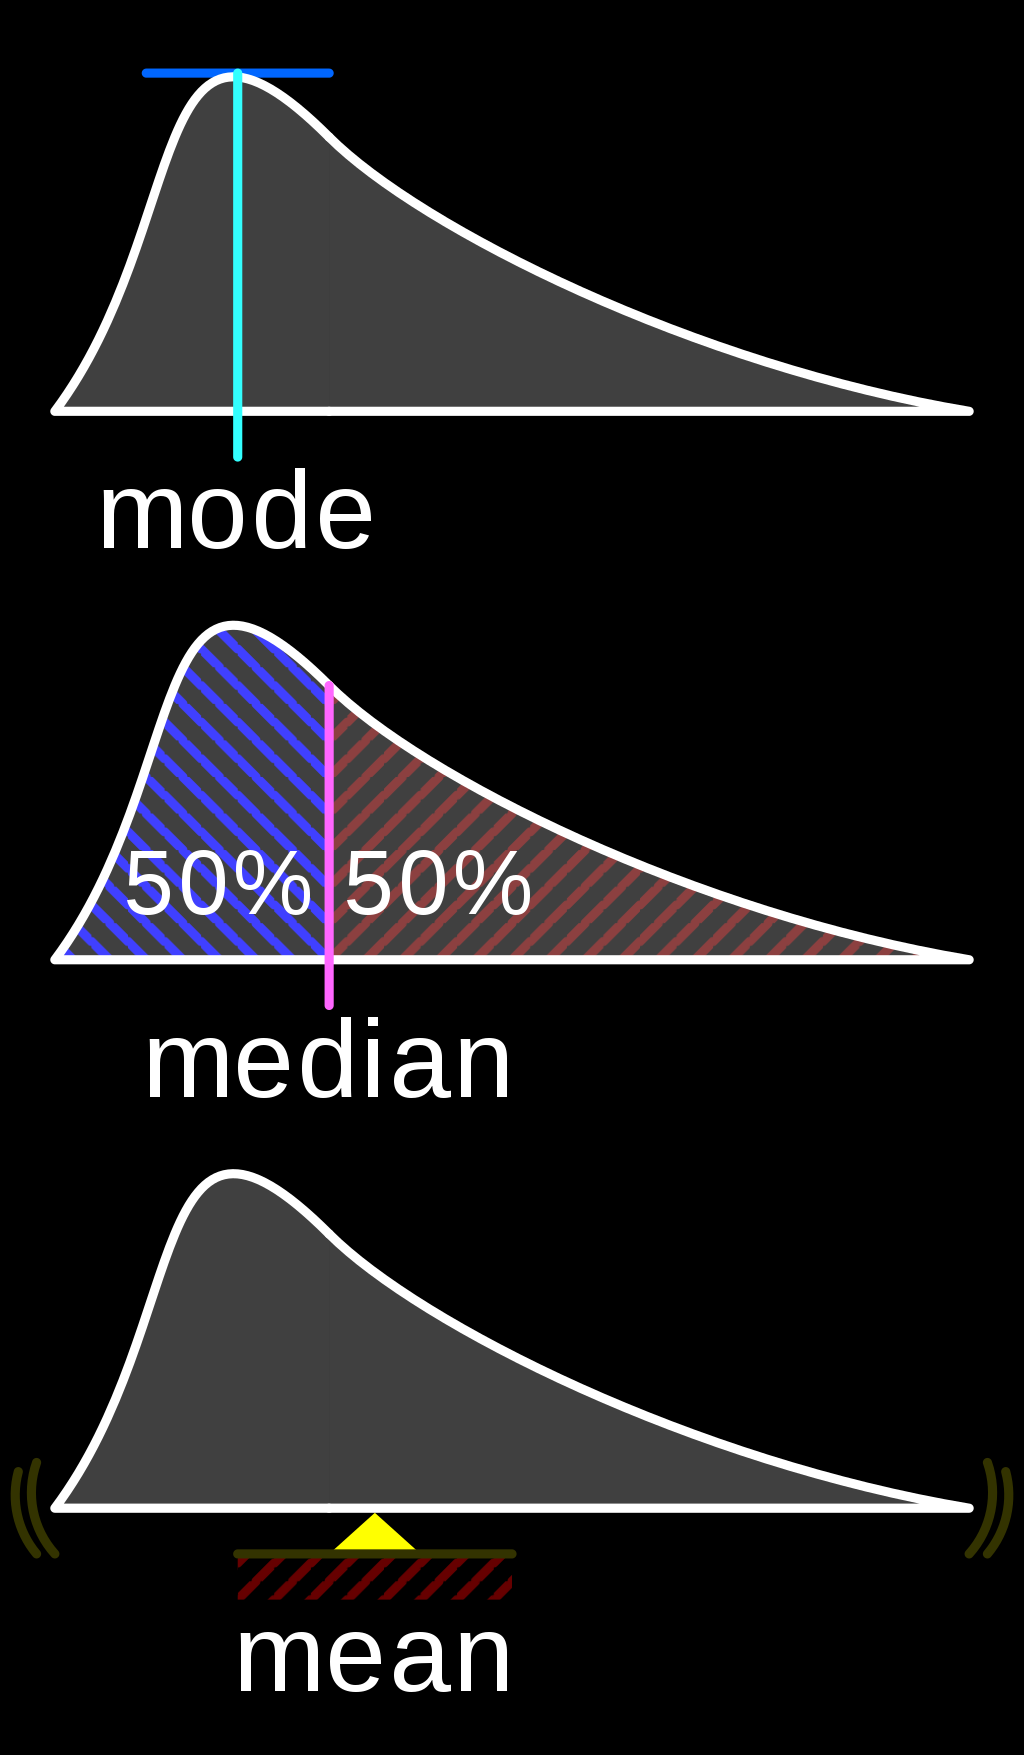
\includegraphics[scale=0.09]{Visualisation_mode_median_mean.svg-neg.png}

\vfill
\footnotesize
\url{https://en.wikipedia.org}
\end{frame}
%-------------- end slide -------------------------------%}}}
%-------------- start slide -------------------------------%{{{ 5. Proof part 1.
\begin{frame}[fragile]

\begin{proofnoend}[ of Part 1. ]
Let $m$ be the \textcolor{magenta}{median} of the random variable $W$. We first claim that
\begin{align}
  \label{E:Median}\tag{$\star$}
  \E(|W-m|)\le \E(|W|).
\end{align}
For any constant $b\in\R$, because
\begin{align*}
  \frac{1}{2} =\bbP(W\le m) = \bbP(W-b\le m-b)
\end{align*}
we see that $m-b$ is the \textcolor{magenta}{median} of $W-b$. Hence, by \eqref{E:Median},
\begin{align*}
  \E\left(|W-m|\right) =\E\left(|(W-b)-(m-b)|\right) \le \E\left(|W-b|\right),\quad \text{for all $b\in\R$},
\end{align*}
which proves the statement.
\end{proofnoend}
\end{frame}
%-------------- end slide -------------------------------%}}}
%-------------- start slide -------------------------------%{{{ 5. Proof of part 1.
\begin{frame}[fragile]
\begin{proofnoend}[ of Part 1. continued ]
It remains to prove \eqref{E:Median}. Without loss of generality, we may assume $m>0$. Then
\begin{align*}
  \E(|W-m|) & = \int_\R |w-m|f_W(w)dw \\
            & = \int_{-\infty}^m (m-w)f_W(w)dw + \int_m^\infty(w-m)f_W(w)dw\\
            & = - \int_{-\infty}^m wf_W(w)dw + \int_m^\infty w\: f_W(w)dw + \frac{1}{2}(m-m)\\
            & = - \int_{-\infty}^0 wf_W(w)dw - \underbrace{\int_{0}^m wf_W(w)dw}_{\ge 0}  + \int_m^\infty w\: f_W(w)dw \\
            & \le - \int_{-\infty}^0 wf_W(w)dw   + \int_{\alert{0}}^\infty w\: f_W(w)dw \\
            & = \int_{\R} |w| f_W(w)dw \\
            & = \E(|W|).
  \end{align*}
  \myQED
 \end{proofnoend}
\end{frame}
%-------------- end slide -------------------------------%}}}
%-------------- start slide -------------------------------%{{{ 5. Proof of part 2.
\begin{frame}[fragile]
  \begin{proofnoend}[ of Part 2. ]
    Let $\mu$ be the \textcolor{yellow}{mean} of  $W$. Then for any $b\in\R$, we see that
     \begin{align*}
      \E\left[(W-b)^2\right] & = \E\left[\left([W-\mu]+[\mu-b]\right)^2\right] \\
                             & = \E\left[(W-\mu )^2\right] + 2 (\mu-b)\underbrace{\E(W-\mu)}_{=0} +[\mu-b]^2 \\
                             & = \E\left[(W-\mu )^2\right] +[\mu-b]^2 \\[1em]
                             & \ge  \E\left[(W-\mu )^2\right],
    \end{align*}
    that is,
\begin{align*}
       \E\left[(W-\mu)^2\right] \le  \E\left[(W-b)^2\right], \quad \text{for all $b\in\R$.}
\end{align*}
    \myQED
  \end{proofnoend}
\end{frame}
%-------------- end slide -------------------------------%}}}
%-------------- start slide -------------------------------%{{{ 5.109
\begin{frame}

\begin{enumerate}
\item[E.g. 1'.]
\begin{minipage}{0.45\textwidth}
\begin{eqnarray*}
 X_1,\cdots, X_n \:\big| \theta &\sim &\text{Bernoulli$(\theta)$}\\
 \Theta & \sim& \text{Beta$(r,s)$}\\
 && \text{$r$ \& $s$ are known}
\end{eqnarray*}
\end{minipage}
\hfill
\begin{minipage}{0.45\textwidth}
\begin{eqnarray*}
 X=\sum_{i=1}^nX_i \: \bigg| \theta&\sim& \text{Binomial$(n,\theta)$}\\
 \Theta & \sim& \text{Beta$(r,s)$}\\
 && \text{$r$ \& $s$ are known}
\end{eqnarray*}
\end{minipage} \pause\pause
\vfill
Prior Beta$(r,s)$ $\rightarrow$ posterior Beta$(k+r, n-k+s)$\\ \pause
upon observing $X=k$ for a random sample of size $n$.  \\[1em] \pause
Consider the $L^2$ loss function.
 \begin{align*}
 \theta_e & =\text{mean of Beta$(k+r,n-k+s)$} \\ \pause
 &= \frac{k+r}{n+r+s}\\ \pause
 &= \frac{n}{n+r+s}\times \underbrace{\mystrut{1em}\left(\frac{k}{n}\right)}_{\text{MLE}} + \frac{r+s}{n+r+s} \times \underbrace{\left(\frac{r}{r+s}\right)}_{\text{Mean of Prior}}
 \end{align*}
 \end{enumerate}
 \end{frame}
%-------------- end slide -------------------------------%}}}
%-------------- start slide -------------------------------%{{{ MLE vs. Prior
\begin{frame}[fragile]
\begin{center}
  MLE vs. Prior

 
\includegraphics[scale=0.25]{./Codes/tug_war.png}
\end{center}
\[\theta_e\]
\[||\]
\begin{align*}
 \frac{n}{n+r+s}\times \underbrace{\mystrut{1em}\left(\frac{k}{n}\right)}_{\text{MLE}} + \frac{r+s}{n+r+s} \times \underbrace{\left(\frac{r}{r+s}\right)}_{\text{Mean of Prior}}
 \end{align*}
\end{frame}
%-------------- end slide -------------------------------%}}}
%-------------- start slide -------------------------------%{{{ 5.110
\begin{frame}
\begin{enumerate}
 \item[E.g. 2'.]
\begin{minipage}{0.45\textwidth}
\begin{eqnarray*}
 X_1,\cdots, X_n \:\big| \theta &\sim &\text{Poisson$(\theta)$}\\
 \Theta & \sim& \text{Gamma$(s,\mu)$}\\
 && \text{$s$ \& $\mu$ are known}
\end{eqnarray*}
\end{minipage}
\hfill
\begin{minipage}{0.45\textwidth}
\begin{eqnarray*}
 W=\sum_{i=1}^nX_i \: \bigg| \theta&\sim& \text{Poisson$(n\theta)$}\\
 \Theta & \sim& \text{Gamma$(s,\mu)$}\\
 && \text{$s$ \& $\mu$ are known}
\end{eqnarray*}
\end{minipage} \pause
\vfill
Prior Gamma$(s,\mu)$ $\rightarrow$ Posterior Gamma$(w+s,\mu+n)$ \\ \pause
 upon observing $W=w$ for a random sample of size $n$.  \\[1em] \pause
Consider the $L^2$ loss function.
 \begin{align*}
 \theta_e & =\text{mean of Gamma$(w+s,\mu+n)$} \\ \pause
 &= \frac{w+s}{\mu +n}\\ \pause
 &= \frac{n}{\mu+n}\times \underbrace{\mystrut{1em}\left(\frac{w}{n}\right)}_{\text{MLE}} + \frac{\mu}{\mu+n} \times \underbrace{\left(\frac{s}{\mu}\right)}_{\text{Mean of Prior}}
 \end{align*}
 \end{enumerate}
\end{frame}
%-------------- end slide -------------------------------%}}}
%-------------- start slide -------------------------------%{{{ MLE vs. Prior
\begin{frame}[fragile]
\begin{center}
  MLE vs. Prior

 
\includegraphics[scale=0.25]{./Codes/tug_war.png}
\end{center}
\[\theta_e\]
\[||\]
\begin{align*}
 \frac{n}{\mu+n}\times \underbrace{\mystrut{1em}\left(\frac{w}{n}\right)}_{\text{MLE}} + \frac{\mu}{\mu+n} \times \underbrace{\left(\frac{s}{\mu}\right)}_{\text{Mean of Prior}}
 \end{align*}
\end{frame}
%-------------- end slide -------------------------------%}}}
%-------------- start slide -------------------------------%{{{ 5.111
\begin{frame}{Appendix: Beta integral}

	 {\bf Lemma.~} $\quad \displaystyle B(\alpha,\beta): = \int_0^1 x^{\alpha-1}(1-x)^{\beta-1}\ud x = \frac{\Gamma(\alpha)\Gamma(\beta)}{\Gamma(\alpha+\beta)}$
	 \vfill
	 {\bf Proof.}
 Notice that
 \[
 \Gamma(\alpha) = \int_0^\infty x^{\alpha-1}e^{-x}dx
 \quad\text{and}\quad
 \Gamma(\beta) = \int_0^\infty y^{\beta-1}e^{-y}dy.
 \]
 Hence,
 \[
 \Gamma(\alpha)\Gamma(\beta)
 = \int_0^\infty\int_0^\infty x^{\alpha-1}y^{\beta-1}e^{-(x+y)}dxdy.
 \]
 \end{frame}

 \begin{frame}
 The key in the proof is the following change of variables:
\vfill
 \[
 \begin{cases}
 x = r^2 \cos^2(\theta)\\
 y = r^2 \sin^2(\theta)
 \end{cases}
 \]
\vfill
 \[
 \Longrightarrow \quad
	 \frac{\partial (x,y)}{\partial (r,\theta)}
 =\begin{pmatrix}
   2r \cos^2(\theta) & 2r\sin^2(\theta) \\
   -2r^2 \cos(\theta)\sin(\theta) & 2r^2 \cos(\theta)\sin(\theta)
  \end{pmatrix}
 \]
\vfill
 \[
 \Longrightarrow \quad \left|\det\left(
 \frac{\partial (x,y)}{\partial (r,\theta)}\right)
 \right| = 4r^3 \sin(\theta)\cos(\theta).
 \]
 \end{frame}
%-------------- end slide -------------------------------%}}}
%-------------- start slide -------------------------------%{{{ 5.112
\begin{frame}
 Therefore,
  \begin{align*}
 \Gamma(\alpha)\Gamma(\beta)
 = &
 \int_0^{\frac{\pi}{2}}d\theta \int_0^\infty dr \:
 r^{2(\alpha+\beta)-4} e^{-r^2} \cos^{2\alpha-2}(\theta)\sin^{2\beta-2}(\theta) \times \underbrace{4 r^3 \sin(\theta) \cos(\theta)}_{\text{Jacobian}}\\
 = & 4 \left(\int_0^{\frac{\pi}{2}}
 \cos^{2\alpha-1}(\theta)\sin^{2\beta-1}(\theta)d\theta \right)
 \left(\int_0^\infty r^{2(\alpha+\beta)-1}e^{-r^2}dr\right).
 \end{align*}
 \vfill
 Now let us compute the following two integrals separately:
\vfill

\begin{align*}
	I_1 &:=\int_0^{\frac{\pi}{2}}
 \cos^{2\alpha-1}(\theta)\sin^{2\beta-1}(\theta)d\theta
 \\[1em]
	I_2 &:= \int_0^\infty r^{2(\alpha+\beta)-1}e^{-r^2}dr
\end{align*}

\end{frame}
%-------------- end slide -------------------------------%}}}
%-------------- start slide -------------------------------%{{{ 5.113
\begin{frame}
For $I_2$, by change of variable $r^2 = u$ (so that $2rdr =du$),
\vfill
\begin{align*}
	I_2 &  =
\int_0^\infty r^{2(\alpha+\beta)-1}e^{-r^2}dr\\
&= \frac{1}{2}\int_0^\infty r^{2(\alpha+\beta)-2}e^{-r^2} \underbrace{2rdr}_{=du}\\
&= \frac{1}{2}\int_0^\infty u^{\alpha+\beta-1}e^{-u}du\\
&=\frac{1}{2} \Gamma(\alpha+\beta).
\end{align*}
\end{frame}
%-------------- end slide -------------------------------%}}}
%-------------- start slide -------------------------------%{{{ 5.114
\begin{frame}
For $I_1$, by the change of variables $\sqrt{x}=\cos(\theta)$ (so that $-\sin(\theta)d\theta = \frac{1}{2\sqrt{x}}dx$),
\vfill
\begin{align*}
I_1 &=
\int_0^{\frac{\pi}{2}}
 \cos^{2\alpha-1}(\theta)\sin^{2\beta-1}(\theta)d\theta
\\ & =  \int_0^{\frac{\pi}{2}}
 \cos^{2\alpha-1}(\theta)\sin^{2\beta-2}(\theta) \times \underbrace{\sin(\theta)d\theta}_{=-\frac{1}{2\sqrt{x}}dx} \\
&= \int_1^0  x^{\alpha-\frac{1}{2}}(1-x)^{\beta-1} \: \frac{-1}{2\sqrt{x}}dx\\
&= \frac{1}{2}\int_0^1  x^{\alpha-1}(1-x)^{\beta-1} \: dx
\\& = \frac12 B(\alpha,\beta)
\end{align*}
\end{frame}
%-------------- end slide -------------------------------%}}}
%-------------- start slide -------------------------------%{{{ 5.115
\begin{frame}
Therefore,
\begin{align*}
	\Gamma(\alpha) \Gamma(\beta) & = 4 I_1 \times I_2 \\
				     &= 4 \times \frac12 \Gamma(\alpha+\beta) \times \frac12 B(\alpha,\beta)
\end{align*}
i.e.,
\[
	B(\alpha,\beta) = \frac{\Gamma(\alpha)\Gamma(\beta)}{\Gamma(\alpha+\beta)}.
\]
\myEnd
\end{frame}
%-------------- end slide -------------------------------%}}}
